\documentclass[conference]{IEEEtran}
\IEEEoverridecommandlockouts

\usepackage{cite}
\usepackage{amsmath,amssymb,amsfonts}
\usepackage{graphicx}
\graphicspath{{figures/}}
\usepackage{booktabs}
\usepackage{siunitx}
\usepackage{textcomp}
\usepackage{xcolor}

\sisetup{group-separator={,}, group-minimum-digits=4}

\begin{document}

\title{Predicting Car Insurance Claims with Machine Learning}

% TODO: add all team members
\author{
\IEEEauthorblockN{Brian Chin}
\IEEEauthorblockA{\textit{Department of Computer Science and Engineering} \\
\textit{University at Buffalo}\\
Buffalo, NY, USA \\
bschin@buffalo.edu}
}

\maketitle

\begin{abstract}
% TODO: write once all six models are in
\end{abstract}

\begin{IEEEkeywords}
insurance claim prediction, logistic regression, XGBoost, SHAP
\end{IEEEkeywords}

\section{Introduction}
% TODO: restate the Phase 1 problem statement

\section{Experimental Setup}

The goal of this project is to predict whether a customer will file a car insurance claim using the binary
target OUTCOME, where 1 indicates that a claim was filed. The dataset contains \num{10000} drivers, and
31.3\% of them filed a claim.

We first split the data randomly into \num{8000} training drivers (31.0\% claim rate) and \num{2000} test
drivers (32.8\% claim rate), with the random seed fixed at 123. The Phase~1 preprocessing steps are applied
after this split: regression imputation of CREDIT\_SCORE and ANNUAL\_MILEAGE, min--max scaling, the
engineered INSURANCE\_RISK, CAR\_AGE and FAMILY features, and one-hot encoding, with the test set aligned to
the training columns. The imputation, scaling and encoding are fitted on the training data only and then
applied to the test set, which keeps information about the test drivers out of training. This leaves 29
features.

Both feature-selection methods are also fitted on the training data only. Random Forest importance
(threshold 0.02) selects 16 features (\emph{RF set}), and forward stepwise selection with logistic
regression, scored by cross-validated ROC-AUC, selects 15 features (\emph{Stepwise set}). Every model is
trained once per feature set.

We then hold out 20\% of the training drivers as a stratified validation set (\num{1600} drivers), leaving
\num{6400} drivers for model training. Logistic regression and XGBoost tune their hyperparameters with
5-fold stratified cross-validation (CV) on these \num{6400} drivers, and the test set is used once, after
tuning. We report accuracy, precision, recall and F1-score for the claim class, and ROC-AUC. Because 67.2\%
of the test drivers did not claim, a model that always predicts ``no claim'' already reaches 67.2\%
accuracy, with zero recall and an ROC-AUC of 0.5. This is the baseline every model must beat.

\section{Logistic Regression}
Logistic regression is commonly used for binary classification problems, which makes it suitable for
predicting whether a customer will file an insurance claim. It uses the sigmoid function to estimate the
probability of a claim, producing an output between 0 and 1. This probability can also be useful for
insurance companies when evaluating customer risk and making pricing decisions.

One of the main advantages of logistic regression is its interpretability. By examining the model coefficients
and odds ratios, we can understand how different features are associated with the likelihood of filing a claim.
This is useful in the insurance industry, where companies may need to explain how certain factors influence
their predictions and pricing decisions. Since all our features are either binary values or scaled between
0 and 1 during preprocessing, they can be used directly in the model. Logistic regression also provides a simple
baseline that we can compare with a more complex model.

\subsection{Training and Tuning}
We used grid search to tune the inverse regularization strength $C$, testing 13 values ranging from
$10^{-3}$ to $10^{3}$, and used cross-validation accuracy to select the best value. A smaller value of $C$
applies stronger regularization, which pushes the coefficients closer to zero. The grid also listed
\texttt{l1\_ratio} values of 0, 0.5 and 1 to compare L2, elastic-net and L1 penalties, but in the
scikit-learn version we used, \texttt{l1\_ratio} only takes effect with the elastic-net penalty, so every
candidate used the L2 penalty.

Table~\ref{tab:lr_tuning} shows the tuning results for both feature sets. Tuning improved the
cross-validation accuracy by only 0.09 percentage points for the RF set, and for the Stepwise set the best
value was the default $C = 1$. This suggests that the default hyperparameters were already performing close
to the best settings for our dataset. This is reasonable because logistic regression is a relatively simple
model, and we have \num{6400} training samples. We also observed that the training, cross-validation, and
test accuracies differ by less than 0.3 percentage points, suggesting that the model is not experiencing
significant overfitting.

\begin{table}[t]
\caption{Logistic Regression Tuning Results}
\label{tab:lr_tuning}
\centering
\begin{tabular}{@{}lcc@{}}
\toprule
 & \textbf{RF set} & \textbf{Stepwise set} \\
\midrule
Best $C$ & 3.16 & 1 \\
Penalty & L2 & L2 \\
Untuned CV accuracy & 0.8494 & 0.8533 \\
Tuned CV accuracy & 0.8503 & 0.8533 \\
Tuned training accuracy & 0.8513 & 0.8537 \\
Tuned test accuracy & 0.8515 & 0.8515 \\
\bottomrule
\end{tabular}
\end{table}

\subsection{Effectiveness}
Table~\ref{tab:metrics} and Fig.~\ref{fig:lr_eval} show the performance of logistic regression on the test
dataset. Both models achieved 85.15\% accuracy, which is about 18 percentage points higher than
the baseline. The ROC-AUC scores are about 0.92, meaning the model has about a 92\% chance of ranking
a randomly selected customer who filed a claim higher than one who did not.

We also noticed that precision, which is around 0.79, is higher than recall, which is around 0.75.
For the RF feature set, the model incorrectly predicted 167 out of 656 customers who actually filed a claim
as non-claimants. At the same time, it incorrectly predicted 130 out of \num{1344} non-claimants as claimants.

Since missing a customer who may file a claim could be more costly for an insurance company, one possible
improvement would be to lower the classification threshold below 0.5. This would allow the model to identify
more potential claimants, although it would likely increase the number of false positives.

Overall, the two feature sets performed almost identically. They have the same accuracy, and the Stepwise
set has slightly higher recall, F1-score and ROC-AUC but slightly lower precision, while using one fewer
feature than the RF set.

\begin{table}[t]
\caption{Test-Set Performance}
\label{tab:metrics}
\centering
\small
\setlength{\tabcolsep}{3pt}
\begin{tabular}{@{}lccccc@{}}
\toprule
\textbf{Model} & \textbf{Acc.} & \textbf{Prec.} & \textbf{Rec.} & \textbf{F1} & \textbf{AUC} \\
\midrule
Always ``no claim'' & 0.6720 & 0.0000 & 0.0000 & 0.0000 & 0.5000 \\
LR (RF set)         & 0.8515 & 0.7900 & 0.7454 & 0.7671 & 0.9213 \\
LR (Stepwise set)   & 0.8515 & 0.7890 & 0.7470 & 0.7674 & 0.9229 \\
XGB (RF set)        & 0.8560 & 0.7866 & 0.7698 & 0.7781 & 0.9212 \\
XGB (Stepwise set)  & 0.8545 & 0.7829 & 0.7698 & 0.7763 & 0.9227 \\
\bottomrule
\end{tabular}
\end{table}

\begin{figure*}[t]
\centering
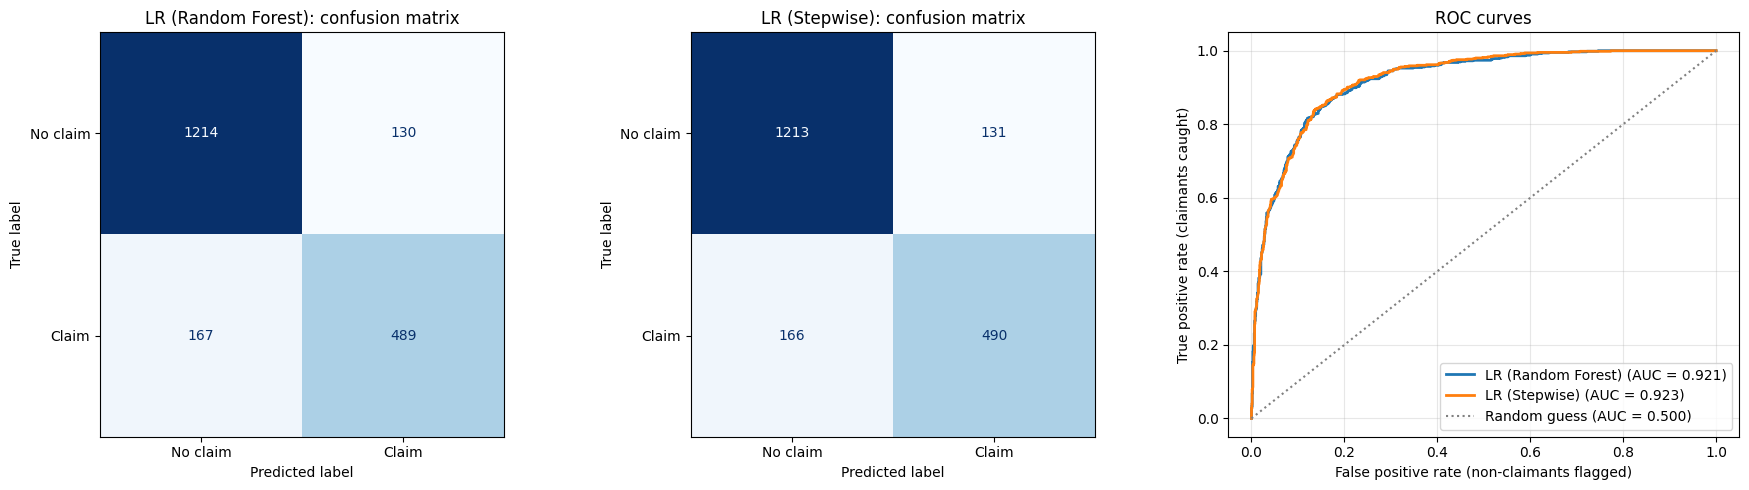
\includegraphics[width=0.9\textwidth]{lr_evaluation.png}
\caption{Logistic regression on the test set: confusion matrices for each feature set and their ROC curves.}
\label{fig:lr_eval}
\end{figure*}

\subsection{Insights}

Fig.~\ref{fig:lr_coef} shows the coefficients from the tuned logistic regression models, while
Table~\ref{tab:odds} shows their corresponding odds ratios, calculated using $e^{\beta}$. Since all features
are scaled between 0 and 1, the odds ratio represents the change in odds when a feature increases from 0 to
1, assuming all other features remain constant. For continuous features, this generally means comparing the
minimum and maximum values.

For categorical features, the odds ratios are compared with the reference categories removed during one-hot
encoding. These reference categories include drivers with 10--19 years of driving experience, female drivers,
vehicles manufactured after 2015, drivers aged 26--39, middle-class income, and postal code 10238.

\begin{figure}[t]
\centering
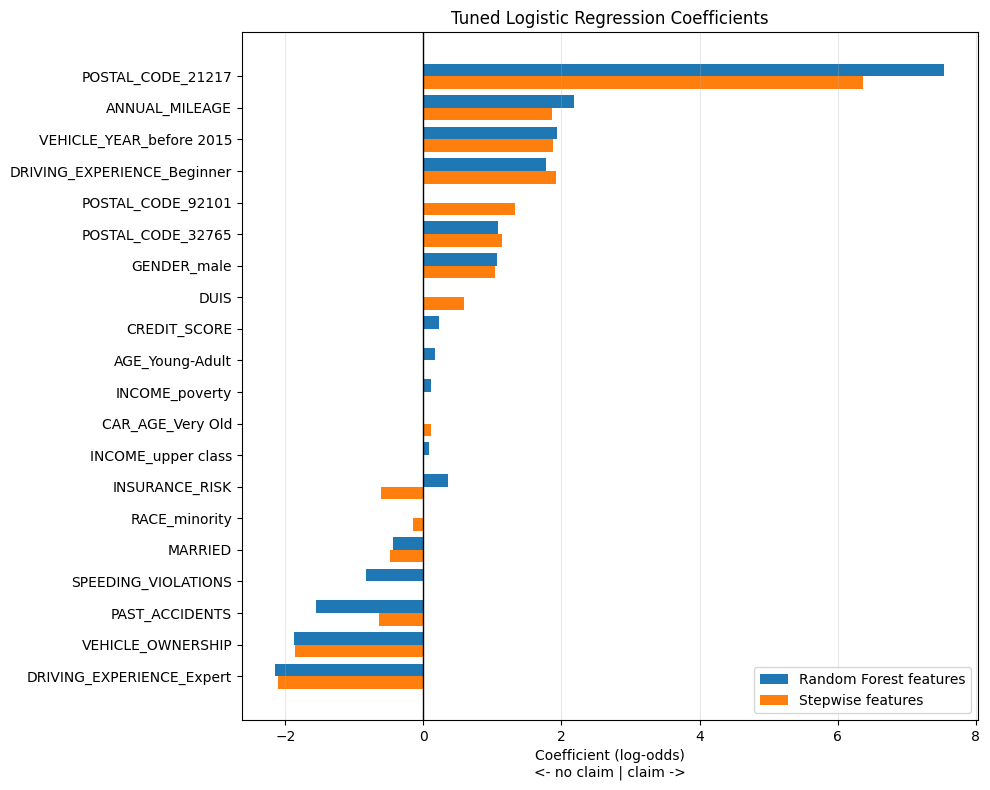
\includegraphics[width=\columnwidth]{lr_coefficients.png}
\caption{Tuned logistic regression coefficients for both feature sets. A missing bar means the feature is not in that set.}
\label{fig:lr_coef}
\end{figure}

\begin{table}[t]
\caption{Logistic Regression Odds Ratios (Selected Features)}
\label{tab:odds}
\centering
\begin{tabular}{@{}lcc@{}}
\toprule
\textbf{Feature} & \textbf{RF set} & \textbf{Stepwise set} \\
\midrule
Annual mileage (max vs.\ min) & 8.93 & 6.48 \\
Driving experience 0--9 yrs & 5.95 & 6.85 \\
Vehicle from before 2015 & 6.95 & 6.54 \\
Postal code 92101 & --- & 3.77 \\
Postal code 32765 & 2.94 & 3.12 \\
Male & 2.91 & 2.81 \\
Married & 0.65 & 0.62 \\
Owns the vehicle & 0.15 & 0.16 \\
Driving experience 20+ yrs & 0.12 & 0.12 \\
\bottomrule
\multicolumn{3}{@{}p{0.9\columnwidth}@{}}{\footnotesize --- = not in this feature set.}
\end{tabular}
\end{table}

\textbf{Driving experience appears to be one of the most important risk factors.} Drivers with 0--9 years of
experience have approximately 6.0--6.9 times the odds of filing a claim compared with drivers who have 10--19
years of experience. On the other hand, drivers with more than 20 years of experience have about 88\%
lower odds of filing a claim. This suggests that driving experience is strongly associated with insurance
claim outcomes.

\textbf{Vehicle characteristics also have a strong relationship with claim risk.} Customers driving vehicles
manufactured before 2015 have approximately 6.5--7 times the odds of filing a claim compared with those
driving newer vehicles. Meanwhile, customers who own their vehicles have around 85\% lower odds of filing a claim.

\textbf{Annual mileage is another important factor.} Customers with the highest annual mileage have
approximately 6.5--9 times the odds of filing a claim compared with those with the lowest mileage. This
suggests that customers who drive more frequently may have a higher chance of making an insurance claim.

Other features also show some relationships with the target. Male drivers have approximately 2.8--2.9 times
the odds of filing a claim compared with female drivers. Customers from postal codes 32765 and 92101 have
around 3--4 times the odds compared with the reference postal code. Meanwhile, married customers have
approximately 35--38\% lower odds of filing a claim.

The remaining demographic features have much smaller effects: credit score (odds ratio 1.25), drivers aged
16--25 (1.18), poverty and upper-class income (1.12 and 1.09), and very old cars (1.12). Race has an odds
ratio of 0.86, suggesting that it has a relatively small effect on the predictions. The driving-record
features are harder to interpret. More past accidents and speeding violations are associated with
\emph{lower} claim odds (odds ratios of 0.21--0.53 and 0.44), while DUIs are associated with higher odds
(1.81). INSURANCE\_RISK even changes direction between the two models (1.43 in the RF set and 0.54 in the
Stepwise set). Because INSURANCE\_RISK is built from the speeding, DUI and past-accident counts, these
features overlap, so their individual coefficients should be read as a group rather than one at a time.

We also noticed that features included in both models generally have similar coefficient values and
directions, with the exception of the overlapping driving-record features. This suggests that the main
relationships identified by logistic regression are fairly consistent across the two feature-selection
methods.

\section{XGBoost}

\subsection{Justification}

XGBoost~\cite{chen2016xgboost} is a gradient-boosted decision tree algorithm that was not covered in class.
It works by building multiple decision trees sequentially, where each new tree attempts to correct the
errors made by the previous trees.

One of the main advantages of XGBoost is its ability to capture complex nonlinear relationships and
interactions between features. For example, the combination of being an inexperienced driver and having
high annual mileage may affect claim risk differently than either feature alone. Unlike logistic regression,
XGBoost can learn these relationships without requiring us to manually create interaction features.

XGBoost also includes L1 and L2 regularization, along with row and column subsampling, which help reduce
overfitting. We chose this algorithm to investigate whether a more complex model could identify additional
patterns in insurance claim behavior that logistic regression might not capture.

\subsection{Training and Tuning}

We used randomized search to tune nine hyperparameters, testing 60 different combinations with 5-fold
cross-validation. The hyperparameters included the number of trees (100--599), learning rate
(0.01--0.3 on a logarithmic scale), maximum tree depth (2--6), minimum child weight (1--9), minimum split
loss $\gamma$ (0--5), row and column subsampling rates (0.6--1.0), and L1/L2 regularization penalties
($10^{-3}$--10 and $10^{-2}$--10 on logarithmic scales).

These ranges were selected based on the default XGBoost settings and the size of our dataset. We used
cross-validation accuracy to select the best hyperparameter combination. Table~\ref{tab:xgb_tuning}
summarizes the tuning results for both feature sets.

\begin{table}[t]
\caption{XGBoost Tuning Results}
\label{tab:xgb_tuning}
\centering
\begin{tabular}{@{}lcc@{}}
\toprule
 & \textbf{RF set} & \textbf{Stepwise set} \\
\midrule
Trees & 573 & 145 \\
Learning rate & 0.10 & 0.035 \\
Max depth & 5 & 4 \\
Min child weight & 6 & 5 \\
$\gamma$ & 2.09 & 3.01 \\
Row / column subsample & 0.93 / 0.72 & 0.71 / 0.64 \\
L1 / L2 penalty & 0.067 / 0.064 & 0.51 / 0.044 \\
\midrule
Untuned CV accuracy & 0.8506 & 0.8522 \\
Tuned CV accuracy & 0.8534 & 0.8553 \\
Tuned training accuracy & 0.8645 & 0.8568 \\
Tuned test accuracy & 0.8560 & 0.8545 \\
\bottomrule
\end{tabular}
\end{table}

From the results, tuning improved the cross-validation accuracy by approximately 0.3 percentage points for
both the RF set and the Stepwise set.

We also noticed that the selected hyperparameters generally favor moderately sized, conservative trees. Both
models use a maximum depth of only 4--5, together with relatively high $\gamma$ values (2.09 and 3.01) and
minimum child weights of 5--6, which make the model more conservative when creating additional splits. The
Stepwise model also uses only 145 trees with a small learning rate of 0.035.

These results suggest that the dataset may not require highly complex tree structures to make accurate
predictions. For the Stepwise set, the training accuracy is less than 0.3 percentage points higher than the
cross-validation and test accuracies. For the RF set, the gap is about one percentage point (0.8645 training
versus 0.8534 cross-validation), which suggests slight overfitting, but the test accuracy (0.8560) remains
close to the cross-validation accuracy.

\subsection{Effectiveness}

Table~\ref{tab:metrics} and Fig.~\ref{fig:xgb_eval} show the performance of XGBoost on the test dataset.
Both models achieved approximately 85.5--85.6\% accuracy, with ROC-AUC scores of 0.921 and 0.923.

Similar to logistic regression, XGBoost has higher precision than recall. Precision is approximately 0.78
to 0.79, while recall is about 0.77 for both feature sets. This means the model fails to identify
approximately 23\% of customers who actually filed a claim.

The confusion matrices show 151 false negatives for both feature sets and 137--140 false positives. Compared
with logistic regression, XGBoost identifies about 15 more of the 656 customers who filed a claim, at the
cost of slightly more false positives.

The RF set has slightly higher accuracy, precision and F1-score, while the Stepwise set has a slightly higher
ROC-AUC. Overall, XGBoost performs well, but its results are very close to those of logistic regression.

\begin{figure*}[t]
\centering
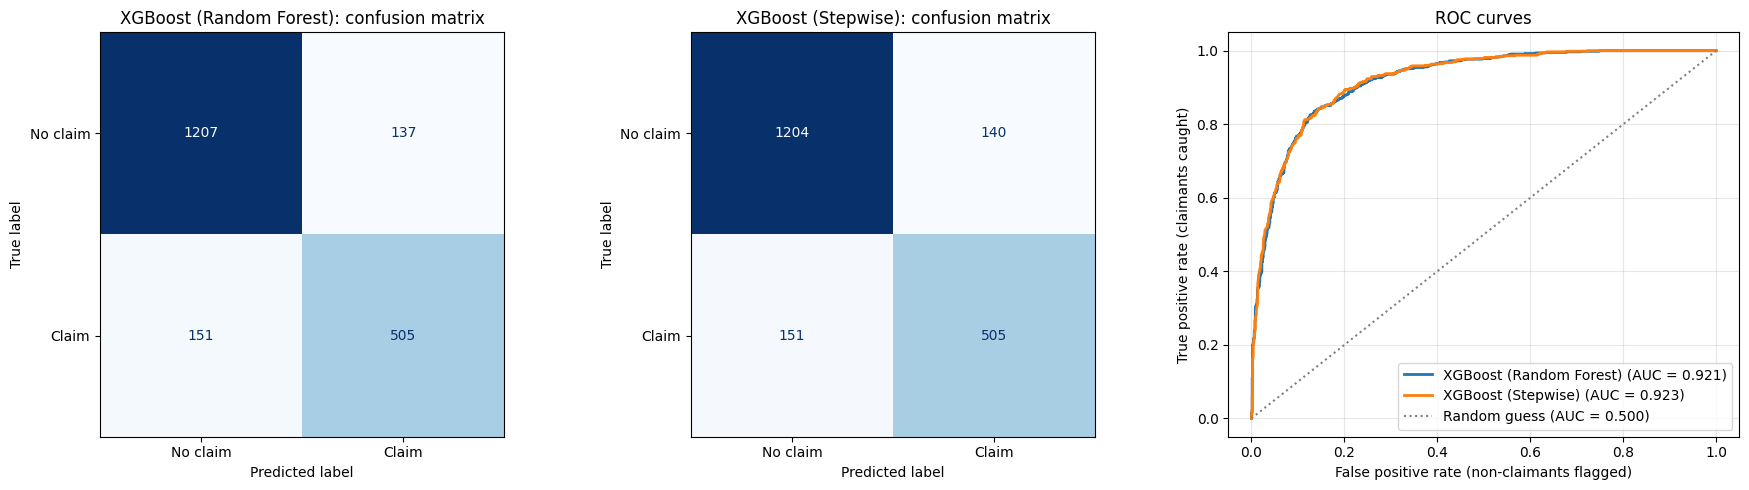
\includegraphics[width=0.9\textwidth]{xgb_evaluation.png}
\caption{XGBoost on the test set: confusion matrices for each feature set and their ROC curves.}
\label{fig:xgb_eval}
\end{figure*}

\subsection{Insights}

To better understand how XGBoost makes its predictions, we used SHAP values~\cite{lundberg2017unified},
which can be calculated exactly for tree models using TreeSHAP~\cite{lundberg2020local}. SHAP explains
each prediction by assigning a contribution value to every feature.

In our model, SHAP values are expressed in log-odds. A positive SHAP value means the feature pushes the
prediction toward filing a claim, while a negative value pushes it toward not filing a claim.

Each prediction starts from the expected model output, $E[f(X)] = -0.83$ for the RF set and $-0.81$ for
the Stepwise set. After converting these log-odds values using the sigmoid function, they correspond to a
baseline claim probability of approximately 30--31\%, which is close to the claim rate in our training data.

\begin{figure*}[t]
\centering
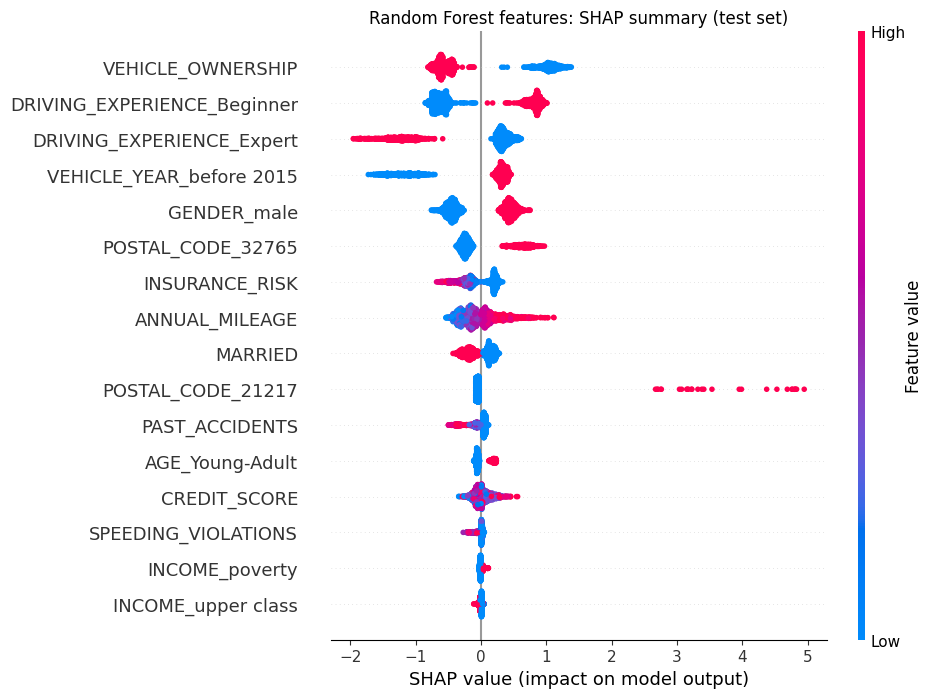
\includegraphics[width=0.48\textwidth]{shap_beeswarm_rf.png}\hfill
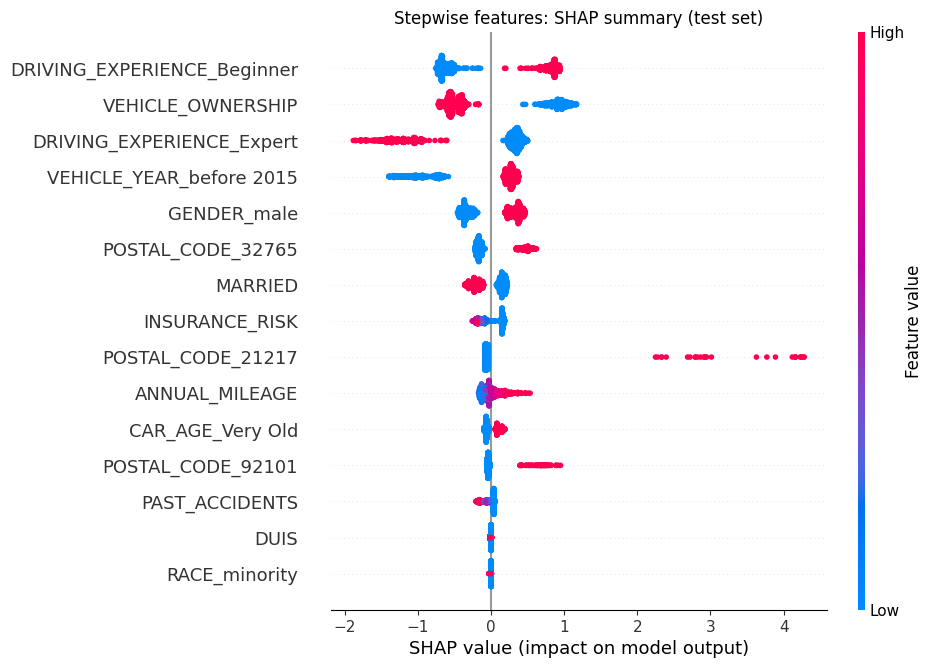
\includegraphics[width=0.48\textwidth]{shap_beeswarm_stepwise.png}
\caption{SHAP summary for the tuned XGBoost models on the test set (left: RF set, right: Stepwise set). Each dot is one driver; color is the feature's value (red = high or 1, blue = low or 0).}
\label{fig:shap_beeswarm}
\end{figure*}

\textbf{Global patterns (Fig.~\ref{fig:shap_beeswarm}).} From the SHAP summary plots, we observed that both
models identify the same five most important features: vehicle ownership, beginner driving experience,
expert driving experience, vehicle year, and gender. The only difference is that vehicle ownership ranks
first for the RF set, while beginner driving experience ranks first for the Stepwise set.

Being a beginner driver increases the model output by approximately +0.8 log-odds, while not being a beginner
decreases it by around $-0.6$. Vehicle ownership also shows a strong relationship with claim predictions.
Customers who own their vehicles generally have negative SHAP values of around $-0.5$, while those who do
not own their vehicles have positive values of approximately +1. Expert drivers have values of around
$-1.3$.

Vehicle year is another important factor. Newer vehicles tend to reduce the predicted claim risk, with SHAP
values of approximately $-0.8$ to $-1.2$. Annual mileage also shows a clear pattern, where higher mileage is
generally associated with higher predicted claim risk. Postal codes 32765 and 92101 push predictions toward
a claim by about +0.4 to +0.9.

On the other hand, features related to driving records, including PAST\_ACCIDENTS,
SPEEDING\_VIOLATIONS, DUIS and INSURANCE\_RISK, have small SHAP values, and higher values of these features
slightly lower the prediction rather than raise it. This is consistent with the logistic regression
results, where these overlapping features had small or unstable coefficients. Race has SHAP values close to
zero, suggesting that it has relatively little influence on the XGBoost predictions.

\begin{figure*}[t]
\centering
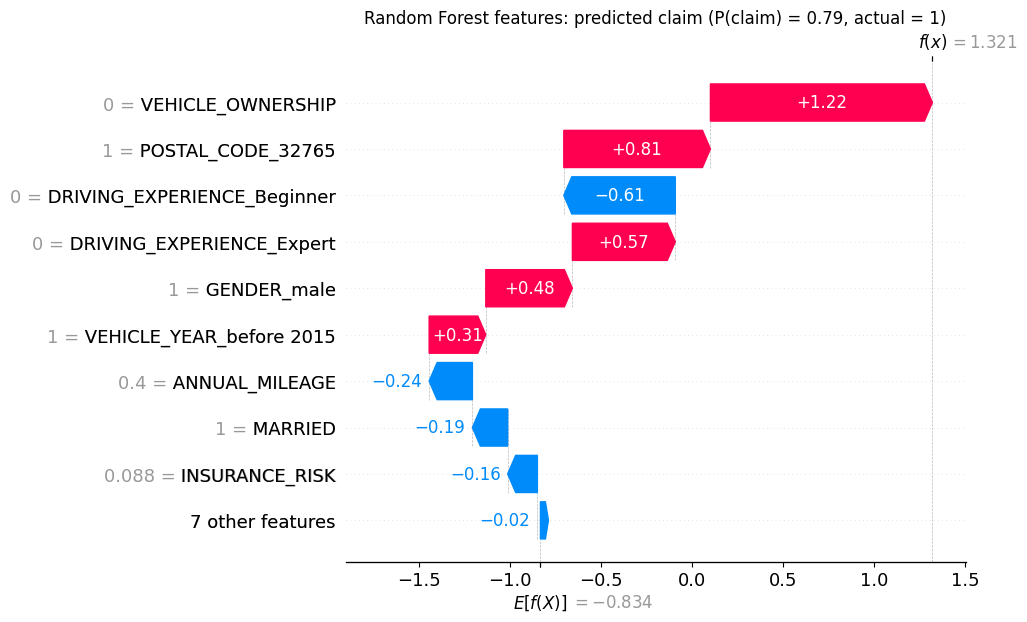
\includegraphics[width=0.48\textwidth]{shap_waterfall_rf_claim.png}\hfill
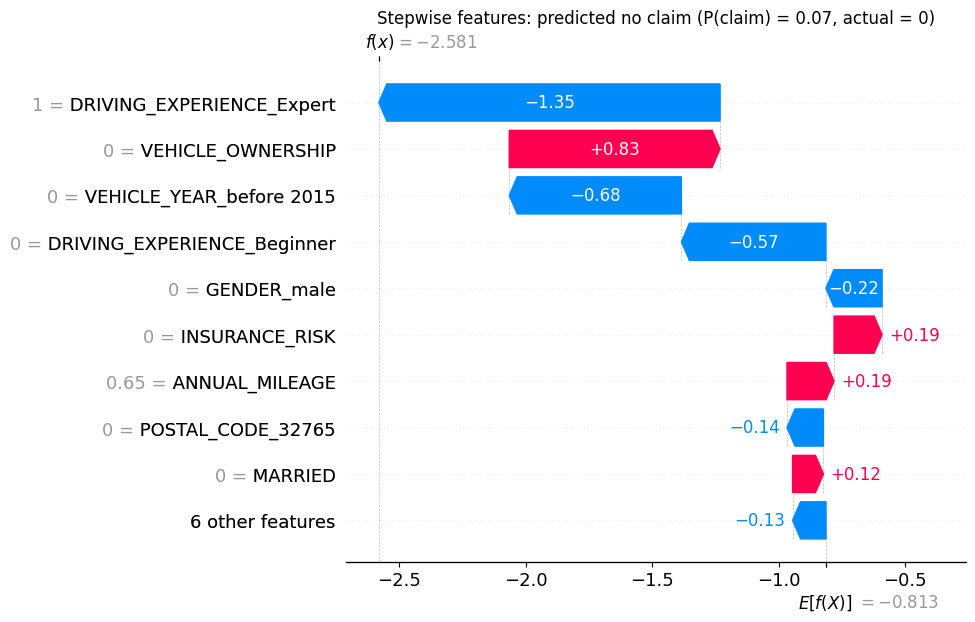
\includegraphics[width=0.48\textwidth]{shap_waterfall_stepwise_noclaim.png}
\caption{SHAP explanations for two individual test drivers. Left: a typical predicted claimant (RF set, $P(\text{claim}) = 0.79$, did claim). Right: a typical predicted non-claimant (Stepwise set, $P(\text{claim}) = 0.07$, did not claim).}
\label{fig:shap_waterfall}
\end{figure*}

\textbf{Individual drivers (Fig.~\ref{fig:shap_waterfall}).} We also used SHAP waterfall plots to
understand how the models make predictions for individual customers.

For the customer who was correctly predicted to file a claim, the largest contribution comes from not
owning the vehicle (+1.22), followed by living in postal code 32765 (+0.81). Not being an expert driver
(+0.57), being male (+0.48) and driving an older vehicle (+0.31) also increase the prediction.
Interestingly, this customer is not a beginner driver, which contributes $-0.61$, but the positive
contributions are much larger than the negative ones, resulting in a predicted claim probability of 79\%.

For the customer who was correctly predicted not to file a claim, the model gives a claim probability of
only 7\%. Interestingly, this customer does not own the vehicle, which contributes +0.83 toward filing a
claim. However, several other features reduce the prediction. These include having expert driving
experience ($-1.35$), driving a newer vehicle ($-0.68$), not being a beginner driver ($-0.57$), and being
female ($-0.22$).

This example shows that even when a customer has one feature associated with higher claim risk, the combined
effects of other features can still result in a low predicted probability.

\section{Comparison of Logistic Regression and XGBoost}
The two algorithms perform almost identically: test accuracy within 0.5 percentage points, ROC-AUC within 0.002, and nearly overlapping ROC curves. XGBoost has slightly higher recall (0.770 versus 0.745--0.747) and F1-score, so it identifies a few more customers who filed a claim, but it does not rank customers by risk any better. XGBoost can model interactions and nonlinear effects, yet it gains very little here, and its tuning favored conservative trees. Together these suggest that claim risk in this dataset is mostly linear and additive in the selected features. The two models also agree on what drives risk: SHAP directions match the signs of the logistic regression coefficients for the major features (vehicle ownership, driving experience, vehicle year, gender, annual mileage, marital status and postal code), and the features with small logistic regression effects are the ones SHAP places near zero. For this problem, logistic regression is the more practical choice: it is almost as accurate, faster to train, and its odds ratios are easier to explain to policyholders and regulators. Neither feature set is consistently better than the other for either algorithm.

\section{Limitations}
\begin{itemize}
\item \textbf{Postal code 21217.} All 74 model-training drivers and all 28 test drivers in this postal code filed a claim, so both models treat it as a near-certain claim (logistic regression odds ratios of about 590--\num{1900}, and the largest SHAP values). This is most likely an artifact of the dataset rather than a real geographic effect, and we do not present it as an insight.
\item \textbf{Driving-record features.} More past accidents and speeding violations are associated with \emph{lower} claim odds, and INSURANCE\_RISK changes direction between the two feature sets. These features overlap with each other, and they are likely confounded with driving experience: experienced drivers have had more years to build up accidents, yet claim less. Our results are associations, not causal effects.
\item \textbf{Penalty tuning.} Because of the scikit-learn version we used, the L1 and elastic-net penalties in the logistic regression grid had no effect, so only L2-regularized models were compared.
\item \textbf{CAR\_AGE feature.} The median annual mileage used to define CAR\_AGE is computed separately for the training and test sets rather than taken from the training set alone. This feature has little influence on our models, so the effect is likely small.
\item \textbf{Fairness.} Gender has a measurable effect on predictions (odds ratio about 2.8--2.9). Using gender in insurance pricing is restricted in some jurisdictions, so a deployed model would need to account for this.
\end{itemize}

% TODO: sections for the other team members' four models

\begin{thebibliography}{00}

\bibitem{chen2016xgboost}
T. Chen and C. Guestrin,
``XGBoost: A scalable tree boosting system,''
in \textit{Proc. 22nd ACM SIGKDD Int. Conf. Knowledge Discovery and Data Mining},
2016, pp. 785--794.

\bibitem{lundberg2017unified}
S. M. Lundberg and S.-I. Lee,
``A unified approach to interpreting model predictions,''
in \textit{Advances in Neural Information Processing Systems 30},
2017, pp. 4765--4774.

\bibitem{lundberg2020local}
S. M. Lundberg \textit{et al.},
``From local explanations to global understanding with explainable AI for trees,''
\textit{Nature Machine Intelligence},
vol. 2, no. 1, pp. 56--67, 2020.

\end{thebibliography}

\end{document}
